\documentclass[tikz,border=8pt]{standalone}
\usepackage{amsmath,amssymb}
\usetikzlibrary{arrows.meta,calc,positioning,decorations.pathmorphing}

\begin{document}
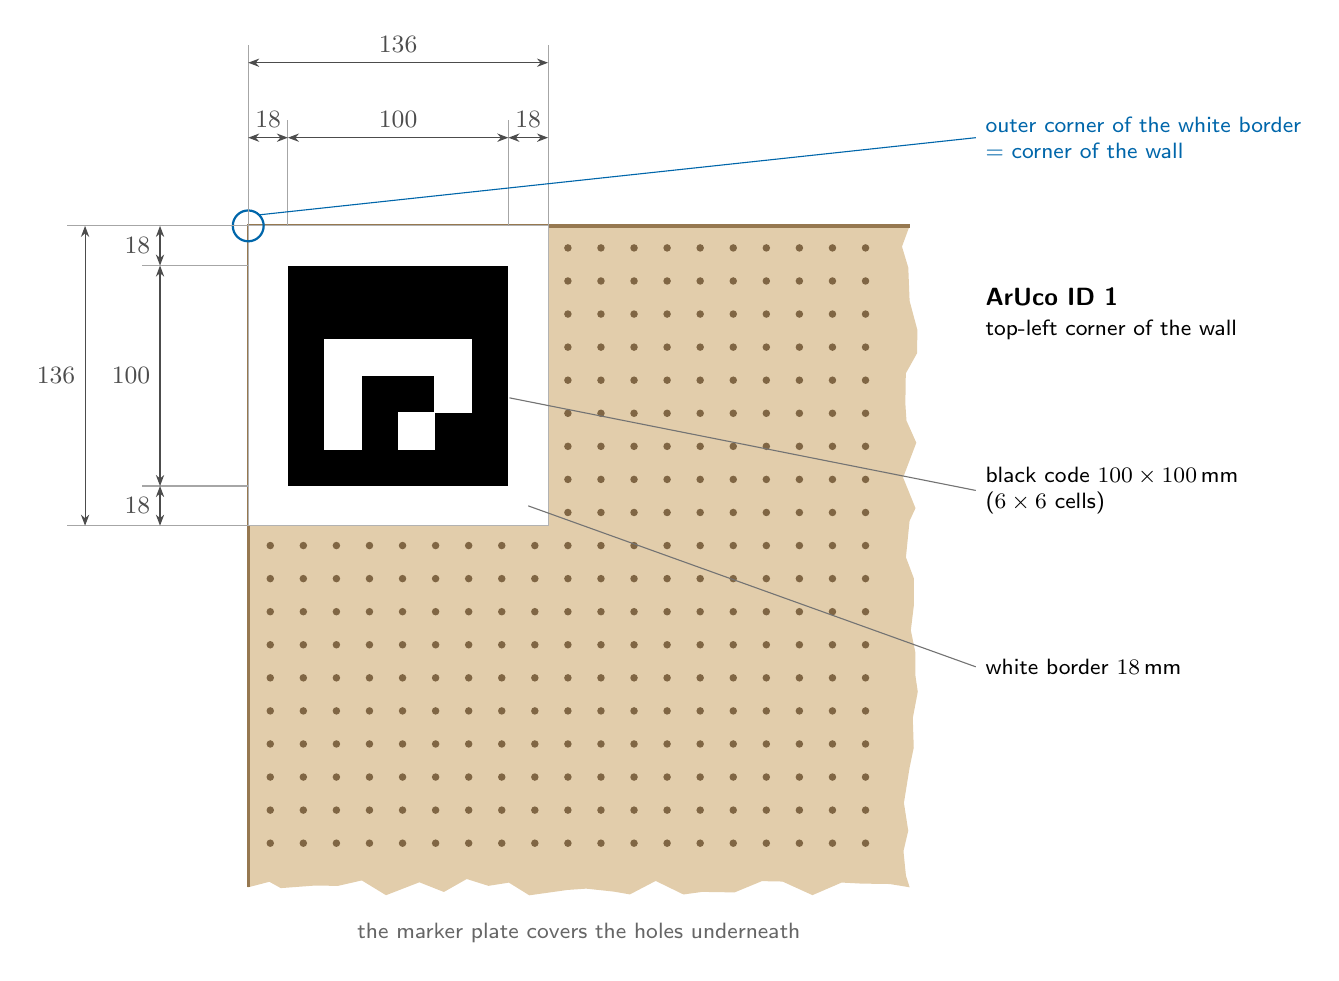
\begin{tikzpicture}[
    x=0.028cm, y=0.028cm,            % 1 unit = 1 mm
    >={Stealth[length=4pt,width=3pt]},
    font=\sffamily\small,
    dim/.style={<->,thin,black!70},
    ext/.style={thin,black!35},
    lead/.style={thin,black!55},
  ]
  \definecolor{wood}{RGB}{226,205,171}
  \definecolor{woodE}{RGB}{150,120,80}
  \definecolor{acc}{RGB}{0,102,170}

  % genuine DICT_4X4_50 patterns (white cells), generated by gen_aruco.py
  % GEN ARUCO BEGIN
  \def\arucoA{1/3,2/3,3/3,4/3,1/2,4/2,1/1,3/1}% ID 1
  \def\arucoB{3/4,4/4,3/3,4/3,3/2,1/1,2/1,4/1}% ID 2
  \def\arucoC{1/4,4/4,1/3,4/3,2/2,2/1,3/1}% ID 3
  \def\arucoD{2/4,4/4,2/3,1/2,4/2,1/1,2/1,3/1}% ID 4
  \def\arucoE{2/4,3/4,4/4,1/3,4/3,1/2,2/2,1/1,2/1,4/1}% ID 5
  % GEN ARUCO END

  % top-left corner of the wall at (0,0); wall extends to +x and -y
  \fill[wood] (0,0) -- (300,0) decorate[decoration={random steps,segment length=9,amplitude=3}]
      {-- (300,-300)} decorate[decoration={random steps,segment length=9,amplitude=3}]
      {-- (0,-300)} -- cycle;
  \foreach \i in {0,...,18}{\foreach \j in {0,...,18}{
      \fill[woodE!85!black] ({10+15*\i},{-10-15*\j}) circle (1.7);}}
  \draw[woodE,very thick] (0,-300) -- (0,0) -- (300,0);

  % marker plate: black code \K + white border \B on each side = \T (mm)
  \def\K{100}\def\B{18}
  \pgfmathtruncatemacro{\T}{\K+2*\B}
  \pgfmathsetmacro{\cs}{\K/6}% cell size
  \fill[white,draw=black!30,line width=0.3pt] (0,0) rectangle (\T,-\T);
  \fill[black] (\B,{-\B-\K}) rectangle ({\B+\K},-\B);
  \foreach \c/\r in \arucoA{
    \filldraw[white,line width=0.3pt] ({\B+\cs*\c},{-\B-\K+\cs*\r}) rectangle ++(\cs,\cs);}

  % wall corner
  \draw[acc,thick] (0,0) circle (7);

  % ---- dimensions: top chain + total
  \draw[ext] (0,0) -- (0,82); \draw[ext] (\T,0) -- (\T,82);
  \draw[ext] (\B,0) -- (\B,48); \draw[ext] ({\B+\K},0) -- ({\B+\K},48);
  \draw[dim] (0,40) -- (\B,40) node[midway,above=0pt] {$\B$};
  \draw[dim] (\B,40) -- ({\B+\K},40) node[midway,above=0pt] {$\K$};
  \draw[dim] ({\B+\K},40) -- (\T,40) node[midway,above=0pt] {$\B$};
  \draw[dim] (0,74) -- (\T,74) node[midway,above=0pt] {$\T$};

  % ---- dimensions: left chain + total
  \draw[ext] (0,0) -- (-82,0); \draw[ext] (0,-\T) -- (-82,-\T);
  \draw[ext] (0,-\B) -- (-48,-\B); \draw[ext] (0,{-\B-\K}) -- (-48,{-\B-\K});
  \draw[dim] (-40,0) -- (-40,-\B) node[midway,left=0pt] {$\B$};
  \draw[dim] (-40,-\B) -- (-40,{-\B-\K}) node[midway,left=0pt] {$\K$};
  \draw[dim] (-40,{-\B-\K}) -- (-40,-\T) node[midway,left=0pt] {$\B$};
  \draw[dim] (-74,0) -- (-74,-\T) node[midway,left=0pt] {$\T$};

  % ---- callouts (outside the wall, on the right)
  \node[anchor=west,align=left] (Lid) at (330,-40)
       {\bfseries ArUco ID 1\\ \footnotesize top-left corner of the wall};
  \node[anchor=west,align=left,font=\sffamily\footnotesize] (Lcode) at (330,-120)
       {black code $\K\times\K$\,mm\\ ($6\times6$ cells)};
  \draw[lead] (Lcode.west) -- ({\B+\K+0.5},{-\B-0.6*\K});
  \node[anchor=west,align=left,font=\sffamily\footnotesize] (Lbord) at (330,-200)
       {white border $\B$\,mm};
  \draw[lead] (Lbord.west) -- ({\T-\B/2},{-\T+\B/2});
  \node[anchor=west,align=left,font=\sffamily\footnotesize,text=acc] (Lcor) at (330,40)
       {outer corner of the white border\\ $=$ corner of the wall};
  \draw[acc,thin] (Lcor.west) -- (5,5);

  \node[anchor=north,font=\sffamily\footnotesize,text=black!60] at (150,-312)
       {the marker plate covers the holes underneath};
\end{tikzpicture}
\end{document}
